\documentclass{report}
\usepackage[utf8]{inputenc}
\usepackage[T1]{fontenc} 
\usepackage[francais]{babel}
\usepackage{colortbl}
\usepackage{amssymb}
\usepackage{pgf, tikz}
\usepackage{xcolor}
\usepackage{array}
    \title{\textit{Rapport} \\ La compression}
    \author{Lucas \textsc{Labadens} \and Isabelle \textsc{Marino} }
    \date{Le \today}
\begin{document}
\maketitle
 

\section*{Introduction}
La compression de données ou codage de source est un processus informatique permettant de transformer un document sous forme binaire en un autre document du même contenant une suite de bit plus courte que le précédent mais pouvant restituer les mêmes informations en utilisant un algorithme de décompression propre à algorithme de compression qui fut utilisé. En d'autres termes, la compression raccourcit la taille des données. La décompression est l'opération inverse de la compression.

Il y a notamment 2 grands types de compression:
\begin{itemize}
\item la compression sans perte de données
\item la compression avec perte de données
\end{itemize}

Un algorithme de compression sans perte restitue après compression et décompression un document strictement identique à l'original. Les algorithmes de compression sans perte sont utiles pour les documents, les archives, les fichiers exécutables ou les fichiers textes.
Pour la compression de données sans perte, on distingue principalement deux types de codage : le codage entropique et le codage algorithmique.

Avec un algorithme de compression avec perte, la suite de bits obtenue après les  compression et décompression est différente de l'originale, mais l'information restituée est très proche. Les algorithmes de compression avec perte sont utiles pour les images, le son et la vidéo.

Les formats de données tels que ZIP, RAR, GZIP, MP3 et JPEG utilisent des algorithmes de compression de données.
La compression est un procédé très utilisé dans la vie courante pour, par exemple, envoyer certains documents par e-mails ou pour le skockage de documents sur disque dur ou cloud center.
  
Le but de notre projet est de compresser des fichiers sans perte de données. 
Nous allons donc vous présenter différents algorithmes de compression sans perte de données que nous avons coder puis tester.

Dans un premier temps nous vous présenterons, entre autre, le codage de Huffman statique et celui de Lempel-Ziv. 
Pour cela nous avons choisit d'utiliser le langage Java pour nous permettre d'avoir des classes structurées et codées les différents algorithmes tout en gardant une structure et des fonctions communes.
 \part*{Algorithme de compression}
\chapter*{Huffman statique}
\section*{Définition et Exemple }
\subsubsection*{Défnition}
Dans chaque langue on peut remarquer que certain caractère apparaisse plus que d'autre et cela vaut aussi pour n'importe quelle langage informatique, et c'est une utilisant cette redondance de caractère que l'algorithme d'Huffman fonctionne.Dans un fichier un caractère est codé sur un octet quelque soit sa fréquence d'apparition l'algorithme d'Huffman va donc codé chaque caractère sur un nombre de bit différent en faisant en sorte que les caractère les plus redondants soit codé sur le moins de place possible.L'algorithme d'Huffman est un codage anthropique car celui-ci nécessite de laisser des informations sur l'arbre de compression utilisé pour compresser le fichier dans le fichier de décompression.
\subsection*{Compression}
La compression est décomposé en plusieurs partit:
\begin{itemize}
\item[-] Une première partit qui consiste a lire une première fois le fichier que l'on veut compresser et à compter le nombre d'apparition de chaque caractère.On considère ensuite que chaque caractère à un poids qui correspond à son nombre d'apparition.On va ensuite procéder à la construction d'un arbre binaire de compression.Dans notre arbre de compression on considère deux choses: les feuilles qui ont un poids et un caractère et les nœuds qui ont un poids et un fils droit et gauche.Ces deux types sont considérer comme des poids.Pour créer notre arbre on va trier nos feuilles  par ordre croissant de poids puis l'on va relier les deux feuilles de poids plus faibles par un nœud de poids égal à la somme du poids des deux feuilles relier ,puis l'on va à nouveau trier notre liste de poids en enlevant les deux feuilles relier et en ajoutant le nœud que l'on vient de créer.On répète ensuite l'opération jusqu'à qu'il ne reste plus qu'un seul poids qui sera donc la racine de notre arbre binaire.

\item[-]Une fois l'arbre créer il faut récupérer les codes de chaque caractère on va donc parcourir l'arbre à partir de la racine.Lorsque l'on va à gauche dans l'arbre(c'est à dire qu'on se rends sur le fils gauche du nœud sur lequel on se trouve) on ajoute le bit 0 et sinon le bit 1.Lorsque l'on arrive sur une feuille le chemin parcourue depuis la racine(c'est à dire la suite de 0 et de 1) correspond au nouveau code du caractère liée à la feuille.

\item Il faut ensuite écrire l'arbre dans le fichier pour que celui-ci puisse être récuperer a la décompression.

\item Il faut ensuite relire le fichier à compresser et réécrire chaque caractère avec les nouveaux codes obtenu précédemment par le parcours de l'arbre.Enfin, et sachant qu'un fichier à un nombre de bit qui est multiple de 8 (les fichiers sont lu comme des suites d'octets et non seulement de bits, 1 octet = 8 bits), alors nous devons compléter le fichier pour pouvoir écrire ce dernier octet.
Nous avons choisit la convention suivante: mettre "1" puis le nombre de "0" nécessaire. 

\end{itemize}
\subsection*{Decompression}
Pour décompresser un fichier comprimer avec l'algorithme d'Huffman statique,il suffit de récupérer l'arbre écrit en début de fichier puis de lire le fichier bit à bit.Si le bit lu est un 0 on se déplace à gauche dans l'arbre et à droite si c'est 1.Lorsqu'on arrive sur une feuille on écrit le caractère correspondant à cette feuille puis l'on retourne à la racine et on recommence l'opération jusqu'à avoir lu entièrement le fichier comprimer.Le chemin menant à une feuille étant unique on retrouve exactement le même fichier qu'au départ.
\subsection*{Exemple}
Prenons un fichier où il est écrit "fanfaronner".Les caractères présent sont 'f','a','r','o',et 'e'.Pour l'instant chaque caractère est codé sur un octet donc le mot pèse 11 octet soit 88 bit.
On crée ensuite une feuille pour chaque caractère que l'on trie par ordre croissant de répétition :
\begin{center}
(o,1) (e,1) (f,2) (a,2) (r,2) (n,3)
\end{center}
On relie ensuite les plus deux feuilles les plus faibles entre eux par un nœuds :
\begin{center}
\begin{tikzpicture}
\node (0) at (0,0) {2};
\node (1) at (-1,-1) {(o,1)};
\node (2) at (1,-1) {(e,1)};
\node (3) at (3,-1/2) {(f,2)};
\node (4) at (5,-1/2) {(a,2)};
\node(5) at (7,-1/2) {(r,2)};
\node(6) at(9,-1/2) {(n,3)};
\draw [-,>=latex,](0)--(1) node[pos=0.6,left, above]{0};
\draw [-,>=latex,](0)--(2) node[pos=0.6,right, above]{1};
\end{tikzpicture}
\end{center}
\paragraph*{}
Puis l'on réitère l'opération, en considérant les nouveaux poids créer jusqu'à n'avoir plus qu'un seul arbre:

étape 2:

\begin{tikzpicture}

\node(1) at(0,0){4};
\node(2) at(-1,-1){2};
\node(3) at (1,-1){(f,2)};
\node(4) at (-2,-2){(o,1)};
\node(5) at(0,-2){(e,1)};
\node (6) at (3,-1) {(a,2)};
\node(7) at (5,-1) {(r,2)};
\node(8) at(7,-1) {(n,3)};
\draw [-,>=latex,](1)--(2) node[pos=0.6,left, above]{0};
\draw [-,>=latex,](2)--(4) node[pos=0.6,left, above]{0};
\draw [-,>=latex,](1)--(3) node[pos=0.6,right, above]{1};
\draw [-,>=latex,](2)--(5) node[pos=0.6,right, above]{1};

\end{tikzpicture}

\paragraph*{}

étape 3 : 


\begin{tikzpicture}

\node(1) at(0,0){4};
\node(2) at(-1,-1){2};
\node(3) at (1,-1){(f,2)};
\node(4) at (-2,-2){(o,1)};
\node(5) at(0,-2){(e,1)};
\node (6) at (3,-1) {(a,2)};
\node(7) at (5,-1) {(r,2)};
\node(8) at(7,-1) {(n,3)};
\node(9) at(4,0) {4};
\draw [-,>=latex,](1)--(2) node[pos=0.6,left, above]{0};
\draw [-,>=latex,](2)--(4) node[pos=0.6,left, above]{0};
\draw [-,>=latex,](1)--(3) node[pos=0.6,right, above]{1};
\draw [-,>=latex,](2)--(5) node[pos=0.6,right, above]{1};
\draw [-,>=latex,](9)--(6) node[pos=0.6,left, above]{0};
\draw [-,>=latex,](9)--(7) node[pos=0.6,right, above]{1};
\end{tikzpicture}
\paragraph*{}

étape 4 : 


\begin{tikzpicture}

\node(1) at(3,0){4};
\node(2) at(2,-1){2};
\node(3) at (4,-1){(f,2)};
\node(4) at (1,-2){(o,1)};
\node(5) at(3,-2){(e,1)};
\node (6) at (7,-1) {(a,2)};
\node(7) at (9,-1) {(r,2)};
\node(8) at(1,0) {(n,3)};
\node(9) at(8,0) {4};
\node (10) at(2,1){7};
\draw [-,>=latex,](1)--(2) node[pos=0.6,left, above]{0};
\draw [-,>=latex,](2)--(4) node[pos=0.6,left, above]{0};
\draw [-,>=latex,](1)--(3) node[pos=0.6,right, above]{1};
\draw [-,>=latex,](2)--(5) node[pos=0.6,right, above]{1};
\draw [-,>=latex,](9)--(6) node[pos=0.6,left, above]{0};
\draw [-,>=latex,](9)--(7) node[pos=0.6,right, above]{1};
\draw [-,>=latex,](10)--(8) node[pos=0.6,left, above]{0};
\draw [-,>=latex,](10)--(1) node[pos=0.6,right, above]{1};
\end{tikzpicture}


étape 5: 


\begin{tikzpicture}

\node(1) at(7,0){4};
\node(2) at(6,-1){2};
\node(3) at (8,-1){(f,2)};
\node(4) at (5,-2){(o,1)};
\node(5) at(7,-2){(e,1)};
\node (6) at (1,0) {(a,2)};
\node(7) at (3,0) {(r,2)};
\node(8) at(5,0) {(n,3)};
\node(9) at(2,1) {4};
\node (10) at(6,1){7};
\node(11) at(4,2){11};
\draw [-,>=latex,](1)--(2) node[pos=0.6,left, above]{0};
\draw [-,>=latex,](2)--(4) node[pos=0.6,left, above]{0};
\draw [-,>=latex,](1)--(3) node[pos=0.6,right, above]{1};
\draw [-,>=latex,](2)--(5) node[pos=0.6,right, above]{1};
\draw [-,>=latex,](9)--(6) node[pos=0.6,left, above]{0};
\draw [-,>=latex,](9)--(7) node[pos=0.6,right, above]{1};
\draw [-,>=latex,](10)--(8) node[pos=0.6,left, above]{0};
\draw [-,>=latex,](10)--(1) node[pos=0.6,right, above]{1};
\draw [-,>=latex,](11)--(9) node[pos=0.6,left, above]{0};
\draw [-,>=latex,](11)--(10) node[pos=0.6,right, above]{1};
\end{tikzpicture}

On obtient donc à partir de cette arbre un nouveaux type de codage pour les caractères du fichier

a='00' \ \ \ \ \ \ \ r ='01' \ \ \ \ \ \ \ n='10' \ \ \ \ \ \ \ f='111' \ \ \ \ \ \ \ o='1100' \ \ \ \ \ \ \ e='1101'

on peut donc maintenant traduire le mot fanfaronner par '111 00 10 111 00 01 1100 10 10 1101 01

En ajoutant le caractère de fin de fichier pour complétez l'octet cela nous renvoie un fichier de 4 octet au lieu de 11 octet, nous avons donc compressez.

\chapter*{Lempel-Ziv}
\section*{Définition }

L'algorithme de compression de Lempel-Ziv est un codage algorithmique.  Le codage algorithmique n’a pas besoin de transmettre des informations autres que le résultat du codage. Donc il n'est pas nécessaire de transmettre dans le fichier compressé un code pour décompresser celui-ci. Il y a ainsi un autre avantage à ce style de compression: la lecture unique du fichier source. En effet, comme l'algorithme ne se base pas sur la récurrence de modèle dans le fichier source, nous pouvons lire et écrire le fichier compressé en même temps, ainsi cette algorithme nécessite une unique lecture du fichier source, ce qui est par ailleurs intéressant lors de la compression de gros fichiers puisque le temps d'exécution est plu rapide. 
Cette algorithme s'applique uniquement aux fichiers binaires, c'est à dire à tout fichier dont les symboles sont représentés par des bits, et par conséquent à tout types de documents. 

\subsubsection{Compression}
Le codage de la compression s'effectue avec un arbre binaire dont les nœuds sont étiquetés par des entiers. Chaque nœud correspond à un entier $i$. 

On débute avec une unique racine étiquetée à 0.

A l'étape i, on part de la racine on lit un bit et on se déplace à gauche ou à droite si cela est possible. On se déplace vers la gauche si on lit un 0 et vers la droite si on lit un 1. Puis on continue de lire bit à bit jusqu'à ne plus pouvoir se déplacer. Lorsque que c'est le cas, on crée un nouveau nœud fils au nœud courant qu'on numérote i et on écrit le numéro du nœud courant sur $\lceil log_{2}(i) \rceil$ suivit du 0 ou 1 que l'on est en train de lire.
On retourne la racine et on passe à l'étape i+1.

Pour compresser, on a fait une fonction qui analyse les bits lus, elle permet de descendre à gauche si on lit un "0" et à droite si on lit un "1", comme expliqué précédemment. Ensuite, si l'on ne peut pas descendre on lit l'entier du nœud courant. Une fonction le traduit en binaire sur le nombre de bit nécessaire. Ce nombre dépend du nombre de nœud présent dans l'arbre, ie $\lceil log_{2}(i) \rceil$ où i est le nombre de nœud dans l'arbre. 
On écrit alors cette traduction puis le dernier bit lu dans le fichier compressé. On répète cette opération jusqu'à ce qu'on ait plus de bit  à lire dans le fichier source.
Enfin, et sachant qu'un fichier à un nombre de bit qui est multiple de 8 (les fichiers sont lu comme des suites d'octets et non seulement de bits, 1 octet = 8 bits), alors nous devons compléter le fichier pour pouvoir écrire ce dernier octet.
Nous avons choisit la convention suivante: mettre "1" puis le nombre de "0" nécessaire. 

\subsubsection{Décompression}
On crée au fur et à mesure de la lecture bit à bit un tableau t à 2 dimensions.  t[i]= [nœud][bit], où nœud et bit sont des entiers, nœuds et le nombre lu à la i ème étape et bit le bit lu juste après. 
On commence en initialisant la première case à  bit=-1 et nœud =-1 , pour pouvoir donner un repère lors de l'écriture de la décompression, il représente la racine de l'arbre de compression.  
A l'étape i, on lit n=$\lceil log_{2}(i) \rceil$ et le bit suivant. On stock alors le nombre écrit sur n et le bit suivant. On regarde la case n du tableau, on lit le bit stocké dans la case n et on regarde nœud de la même façon jusqu'à arriver à la case 0. On écrit dans le fichier décompressé la suite de bit lu au fur et à mesure.

Pour décompresser, nous avons créé une fonction qui me permet de lire bit à bit notre fichier. Nous lisons alors nos bits en fonction de la puissance de 2 souhaitée, puis nous les mettons dans un tableau pour pouvoir les traduire en un entier i. 
Nous trouvons notre puissance de 2 en fonction du nombre de nœuds déjà lus et stockés précédemment.
Une fois l'entier i  trouvé, nous recherchons dans mon tableau à 2 dimensions à partir de i puis regardons la case du père afin de récupérer tous les bits de la suite. Nous les inversons pour les copier dans le fichier décompressé ensuite nous lisons un dernier bit qui sera aussi copié dans le fichier décompressé.
Nous stockons à la fin du tableau ce nouveau nœud, composée de son père (l'entier i) et du dernier bit lu. 
Nous réitérons cette procédure jusqu'à la fin du fichier. 

 
\section*{Exemple}
Nous allons regarder le fichier composé de 2 caractères "ab".

\subsubsection{Compression}
En terme d'octet "ab" est représenté par : 
		01100001 01100010\\
On lit de la façon suivante pour avoir l'arbre ci dessous :
\begin{center}
\begin{tabular}{ c | c | c }
\underline{0}110000101100010 & \underline{0} \underline{1}10000101100010 & \underline{0} \underline{1} \underline{10}000101100010 \\ 

\begin{tikzpicture}
\node (0) at (0,0) {0};
\node (1) at (-2,-1) {1}; 
\draw [->,>=latex,](0)--(1) node[pos=0.6,left, above]{0};
\end{tikzpicture} 
&
\begin{tikzpicture}
\node (0) at (0,0) {0};
\node (1) at (-2,-1) {1}; 
\node (2) at (2,-1) {2};
\draw [->,>=latex,](0)--(1) node[pos=0.6,left, above]{0};
\draw [->,>=latex,](0)--(2) node[pos=0.6,left, above]{1};
\end{tikzpicture} 
& 
\begin{tikzpicture}
\node (0) at (0,0) {0};
\node (1) at (-2,-1) {1}; 
\node (2) at (2,-1) {2};
\node (3) at (1,-2) {3};
\draw [->,>=latex,](0)--(1) node[pos=0.6,left, above]{0};
\draw [->,>=latex,](0)--(2) node[pos=0.6,left, above]{1};
\draw [->,>=latex,](2)--(3) node[pos=0.6,left, above]{0};
\end{tikzpicture}\\

Etape 1 & Etape 2 & Etape 3 \\
\end{tabular}
\end{center}


\begin{center}
\underline{0} \underline{1} \underline{10} \underline{00} \underline{01}  \underline{011} \underline{000} \underline{10}
\\
\begin{tikzpicture}
\node (0) at (0,0) {0};
\node (1) at (-2,-1) {1}; 
\node (2) at (2,-1) {2};
\node (3) at (1,-2) {3};
\node (4) at (-3,-2) {4}; 
\node (6) at (-0.5,-3) {6};
\node (7) at (-3.5,-3) {7}; 
\node (5) at (-1,-2) {5};
\draw [->,>=latex,](0)--(1) node[pos=0.6,left, above]{0};
\draw [->,>=latex,](0)--(2) node[pos=0.6,left, above]{1};
\draw [->,>=latex,](2)--(3) node[pos=0.6,left, above]{0};
\draw [->,>=latex,](5)--(6) node[pos=0.6,left, above]{1};
\draw [->,>=latex,](1)--(4) node[pos=0.6,left, above]{0};
\draw [->,>=latex,](4)--(7) node[pos=0.6,left, above]{0};
\draw [->,>=latex,](1)--(5) node[pos=0.6,left, above]{1};
\end{tikzpicture}
Dernière étape
\end{center}	

Il y a alors dans le fichier compressé (sans les "." et les "|") :\\ 
0|0.1|10.0|01.0|001.1|101.1| 100.0|010.0 
On complète enfin le dernier octet avec 1 et le nombre de 0 nécessaire. 

\subsubsection{Décompression}
Reprenons cet exemple. 
Nous avons donc dans notre fichier compressé :
00110001 00011101 11000010 01000000 \\
Nous avons une liste composé de nœud avec 2 éléments un entier pour le père et un entier pour le bit représenté sur le flèche de l'arbre de compression. Nous initialisons le nœud 0 avec -1 en valeur pour le père et -1 en valeur pour le bit. 
Puis on lit, le nombre d'octet en fonction du nombre de nœud dans la liste (toujours selon les puissance de 2).
Donc au commencement on lit 0 bit car il y a $2^{0}$ nœud dans la liste, alors on ajoute le nœud 1 avec comme père 0 et comme bit le prochain bit lu, ici 0.
On ajoute alors 0 dans le fichier décompressé. \\
On continue, on lit alors le bit 0 qui sera le père et 1. On ajoute le nœud 2 {0,1} 
dans le liste.On ajoute alors 1 dans le fichier décompressé.\\
On lit les bit 10 qu'on traduit en 2 en nombre décimale on ajoute alors le nœud 3 {2, 0}. On parcours alors la liste on la voir le père 2 on lit son bit et on l'ajoute dans le fichier décompressé jusqu'à arrivé au père 0 . On ajoute 1 dans le fichier décompressé. 

On obtient de cette fonction la liste suivante:
\begin{center}
\begin{tabular}{|c|c|c|c|c|c|c|c|c|c|}
\hline
noeud & 0 & 1 & 2 & 3 & 4 & 5 & 6 & 7 & 8 \\
\hline
père & -1 & 0 & 0 & 2 & 1 & 1 & 5 & 4 & 2\\
\hline
bit & -1 & 0 & 1 & 0 & 0 & 1 & 1 & 0 & 0 \\
\hline 
\end{tabular}
\end{center}
 
Pour écrire à l'étape 7, on regarde le père 4 puis le père 1 puis le père 0. 
On récupère leur bit respectif et on les écrit en commençant par le nœud  1 à jusqu'à celui du bit du nœud 7. On obtient alors la suite: 000.
Pour le nœud 8 on obtient la suite: 10. 



\part*{Analyse des performances}
Nous avons choisit un certain nombre de tests identiques à effectuersur chaque algorithme. Nous commençons par des tests avec des suites théoriques puis nous ferons des tests avec des fichiers plus réalistes des fichiers textes(roman) son et image.
 
Tout d'abord un test de compression théorique simple avec un fichier et un seul caractère à l'intérieur, nous avons pris le caractère "0".
Tout d'abord dans le fichier il a y un unique octet de 0, puis nous dupliquons ce a 10 fois, 20 fois ... Et ainsi de suite pour avoir 10 fichiers de 1 octet , 10, 20 ,30 ,...  octet, jusqu'à 10 Mo.
Puis nous continuons avec des suites plus complexes comme une suite périodique composées que de suite de 01, une suite générée aléatoirement et enfin une suite de Champernowne.
La suite de Champernowne consiste en une suite d'entier naturel de 0,1,2,3,4... en base 10. Cela revient à 0,1,00,01,10,11,000... en base 2.   

Pour finir, une dernière comparaison entre les différents algorithmes avec comme fichier la bible, pour pouvoir comparer les performances entre les algorithmes.

Nous utiliserons ces différents tests pour analyser les performances en terme de taux de compression, ainsi qu'en temps d’exécution pour la compression et la décompression. 
\section*{Analyse du taux de compression}
\subsubsection{ Analyse de l'agorithme de Huffman}

\subparagraph*{}
\hspace{-2cm}\begin{tabular}{l | l}
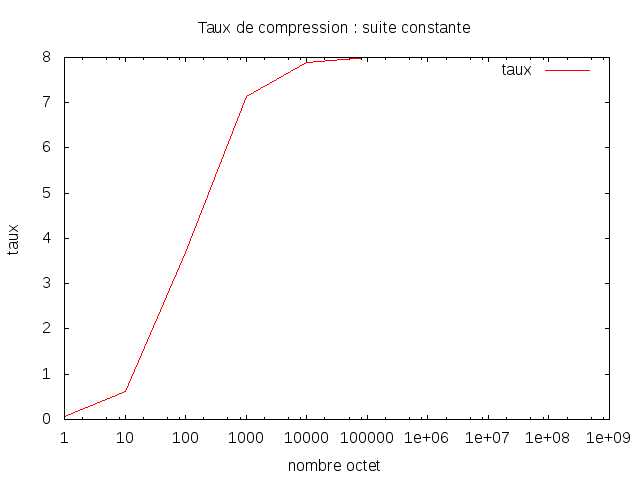
\includegraphics[width=7cm]{HConstant.png} & 
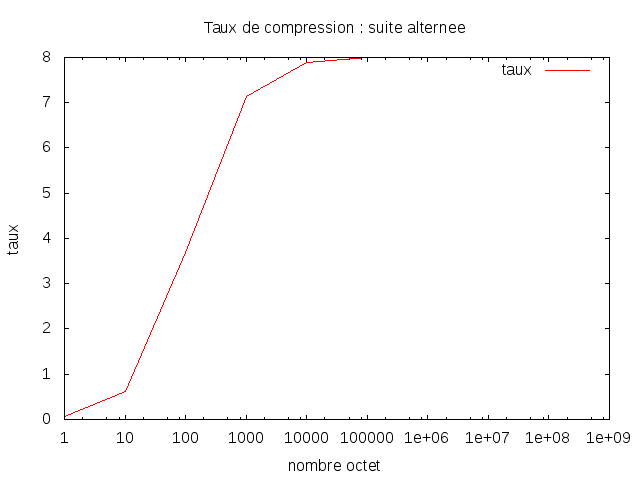
\includegraphics[width=7cm]{alternerH.png}
\end{tabular}


\subparagraph*{}
\hspace{-2cm}\begin{tabular}{l | l}
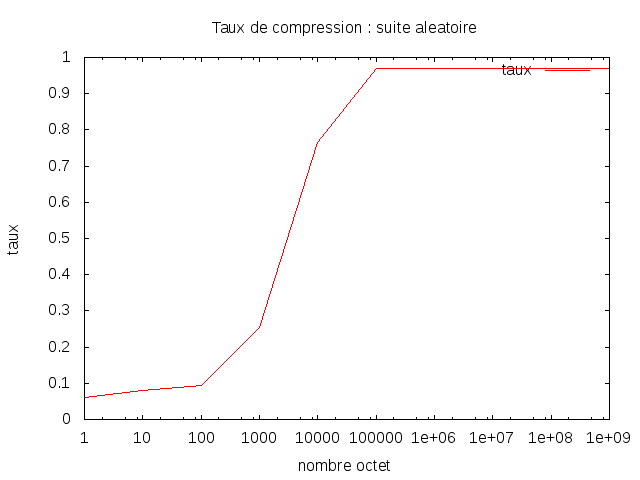
\includegraphics[width=7cm]{aleaH.png} & 
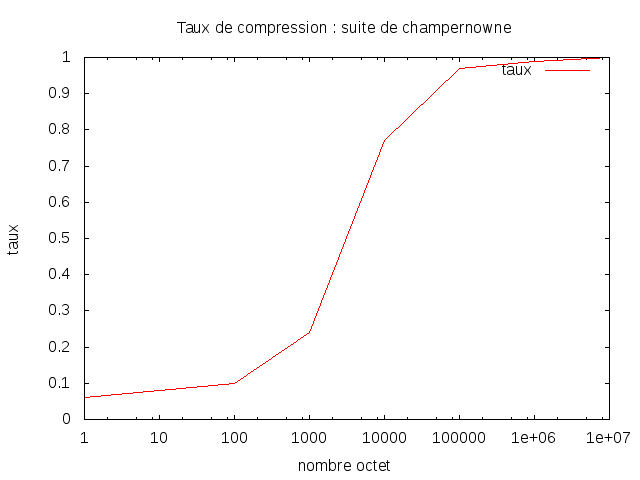
\includegraphics[width=7cm]{champH.png}
\end{tabular}


\subsubsection{ Analyse de l'agorithme de Lemple Ziv}

Tout d'abord regardons nos fichiers composés que de 0, nous obtenons le graphique ci-dessus.
\begin{center}

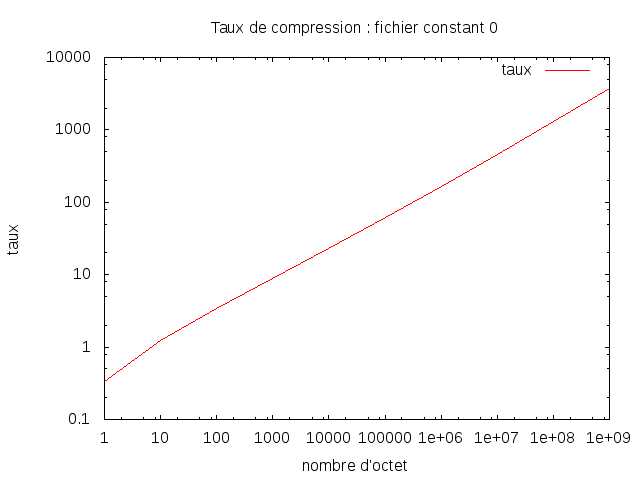
\includegraphics[width=10cm]{LZConstant.png}

\end{center}

On constate que la courbe est logarithmique, plus le nombre d'octet est important plus le taux de compression augmente, ainsi le fichier compressé devient réellement de plus en plus petit. 
On remarque néanmoins que lorsque l'on veut compresser un seul octet le taux de compression est en dessous de 1, c'est-à-dire que le fichier compressé est plus gros que le fichier source. Ceci s'explique notamment par le stockage du premier  octet supplémentaire pour connaître le mode de compression, ici Lempel-Ziv. Il s'explique aussi car le début de compression pour Lempel-Ziv remplace un bit par 2 et ainsi de suite. Nous devons donc attendre les 10 octets dans le fichier source pour que la compression ai vraiment lieu. 
Lors de la compression d'un suite constante comme celle-ci, nous pouvons remarquer que l'arbre de compression est linéaire. En effet, il y a un seule branche composée de 0 les uns à la suite des autres. Le fait qu'il n'y ai qu'une seule branche explique en grande partie la performance de compression pour cette suite. 

\begin{center}
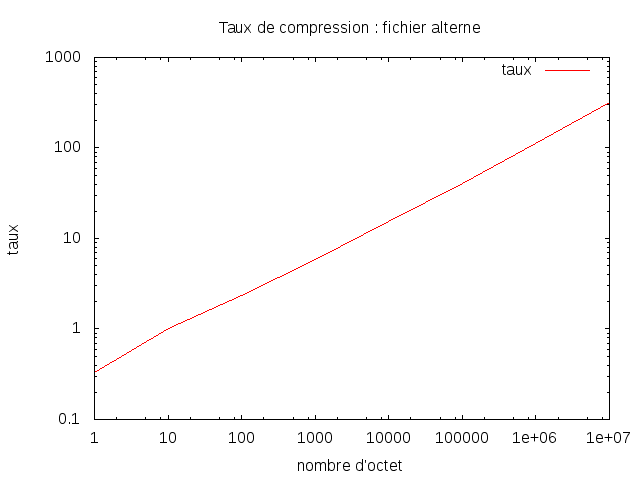
\includegraphics[width=10cm]{LZAlterner.png}
\end{center}

De même que sur le précédent graphique, la suite alternée a une compression dont le taux croît selon la taille de la suite. On constate que sur ce cas, l'arbre de compression quant à lui 2 branches au lieu d'une unique pour le cas constant. Ainsi on observe que la courbe du aux de compression augmente mais qu'elle n'est pas aussi efficace que pour le cas constant, même si l'écart est plutôt faible.
De la même façon que sur la courbe précédente, il faut attendre 10 octets pour qu la compression débute, pour des raisons identiques à celle que nous avons déjà évoquées.  

\begin{center}
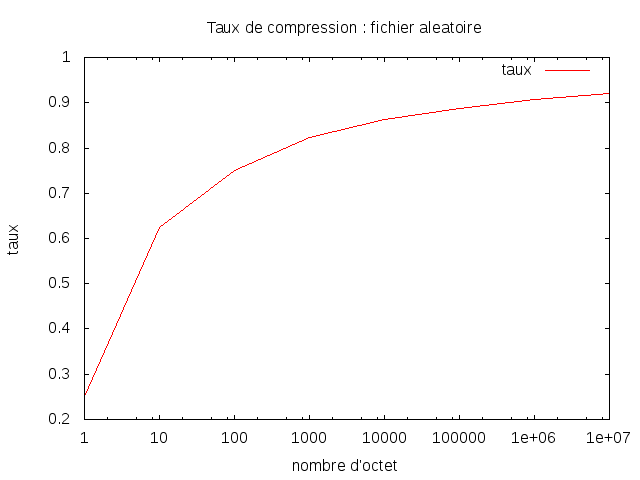
\includegraphics[width=10cm]{LZAleatoire.png}
\end{center}

On observe un changement avec les courbes précédentes, pour une suite aléatoire notre algorithme de compression n'a pas de bon résultat. En effet, le fichier obtenu à un nombre d'octet plus grand que le fichier source peu importe sa taille. Autrement dit, nous algorithme de compression ne compresse pas au contraire. 
On remarque néanmoins que plus le fichier source est grand, plus le taux de compression tend vers 1. Ceci s'explique notamment pas la taille de l'arbre de compression.Plus le fichier source est important, plus il y a de redondance dans les suites d'octets, ainsi on repasse obligatoirement par des chemins déjà existants, qui deviennent au fur et à mesure de plus en plus grand. 
C'est pour cela qu'on observe une courbe qui tend vers 1. 


\begin{center}
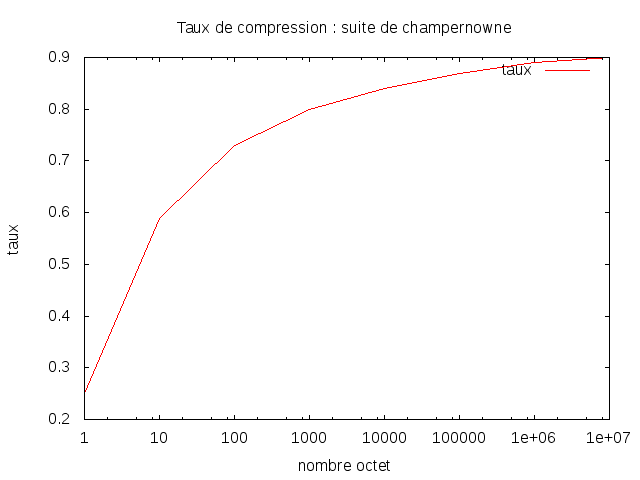
\includegraphics[width=10cm]{champLZ.png}
\end{center}
La suite de Champernowne est une suite très particulière pour notre algorithme. A chaque lecture nous allons créer dans notre arbre de compression un nouveau nœud dont la profondeur sera égal à la hauteur de l'arbre. Lorsque nous avancerons dans le processus, nous créerons tous les nœuds possible dans l'arbre ainsi comme la hauteur de l'arbre ne croîtra pas de façon logarithmique, nous n'aurons pas la possibilité d'avoir une compression satisfaisante. 

\section*{Analyse du temps d’exécution}

\subsubsection*{Compression}
\paragraph*{}
\textbf{Temps d’exécution pour Huffman}
\subparagraph*{}
\hspace{-2cm}\begin{tabular}{l | l}
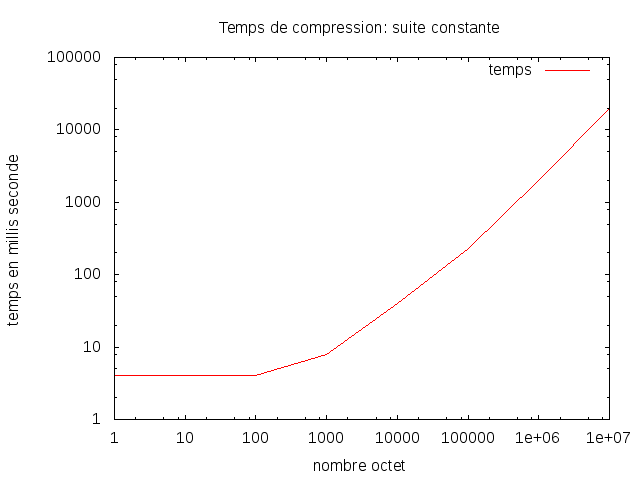
\includegraphics[width=7cm]{tempsChC.png} & 
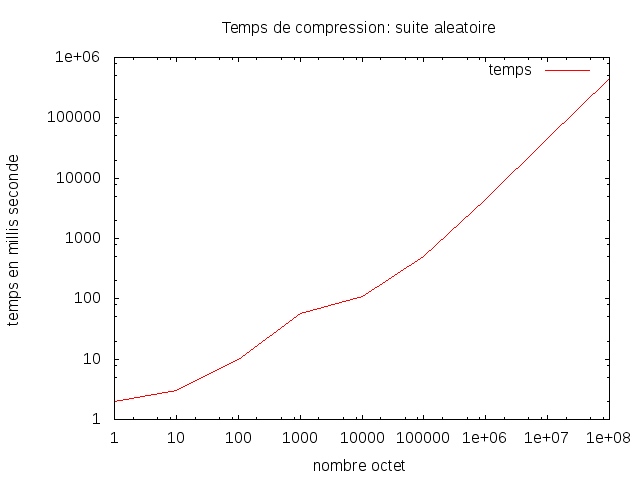
\includegraphics[width=7cm]{tempsChA.png}
\end{tabular}

\subparagraph*{}
Le temps d'exécution pour l’algorithme de Huffman est linéaire, plus le fichier source est important plus le temps d'exécution le devient. Cela est du à la lecture double du fichier source ainsi qu'à la construction de l'arbre. Lorsque le fichier source devient plus grand il faux alors lire beaucoup plus de caractère.    
On constate aussi, que la suite constante nécessite moins de temps pour être compressée que la suite aléatoire. Il y a 2 explications à cela. La première est que le nombre de caractère à comparer est totalement différent par rapport à la suite aléatoire.Il suffit de compter le nombre 0 alors que pour la suite aléatoire il faut compter tous les caractères mais aussi tous les comparer ce qui nécessite plus de temps. La seconde explication découle de la première, en effet pour la suite constante l'arbre de compression ne possède que 2 poids et donc on le copie en un temps plus court qu'un arbre pour complexe comme celui de la suite aléatoire, qui est nécessairement plus grand, voire de taille maximale pour un arbre de Huffman.  

\paragraph*{}
\textbf{Temps d’exécution pour Lempel-Ziv}
\subparagraph*{}
\hspace{-2cm}\begin{tabular}{l | l}
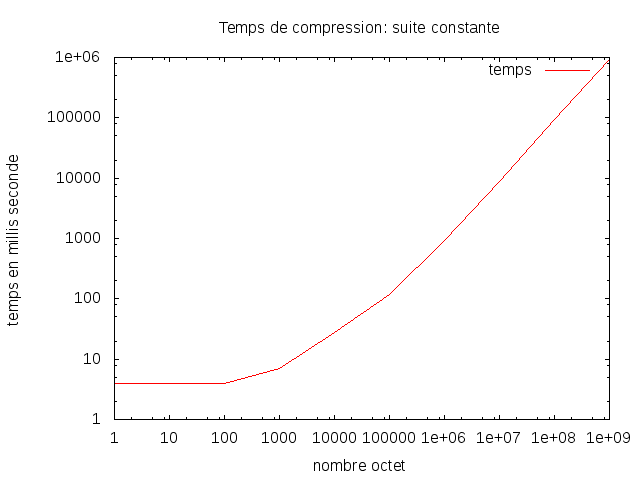
\includegraphics[width=7cm]{tempsClzC.png} & 
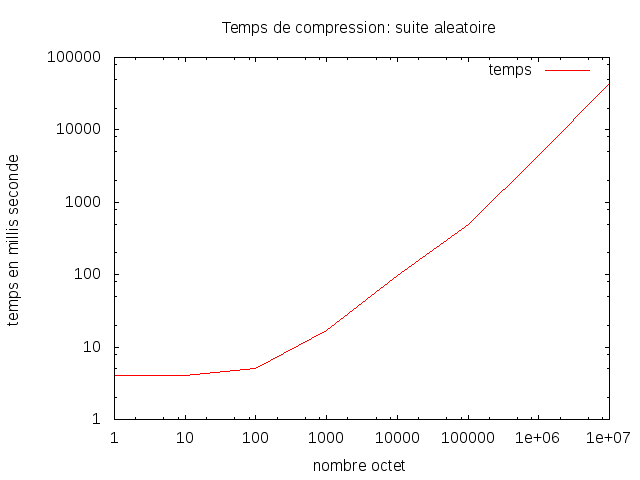
\includegraphics[width=7cm]{tempsClzA.png}
\end{tabular}

\subparagraph*{}
Le temps d'exécution pour l'algorithme de Lempel-Ziv est lui aussi linéaire. De la même façon le temps d'exécution croît en fonction du nombre d'octet présent dans le fichier source. Néanmoins, on remarque que pour la suite constante le temps d'exécution est plus rapide que pour la suite aléatoire. Ceci s'explique notamment par le parcours en profondeur de l'arbre. Dans le cas constant, plus le processus avance et plus le nombre d'octet lu est important avant la création d'un nœud dans l'arbre, le nombre d'octet lu avant la création d'un nœud est logarithmique. Contrairement au cas constant, le cas aléatoire crée des nœuds dans l'arbre de façon plus fréquent, il y a tout simplement moins de redondance dans le fichier source. Ainsi la création de ces multiples nœuds prend plus de temps, c'est donc une conséquence de la différence du temps d'exécution.

\paragraph*{}
En comparaison, les 2 algorithmes présentent des courbes pour le temps d'exécution linéaire. Néanmoins, l'algorithme de Lempel-Ziv a un temps d'exécution pour la compression plus rapide que pour celui de l'algorithme de Huffman. On l'observe de façon très significative dans la cas de la suite constante. Cette différence de rapidité est du à la lecture unique du fichier pour l'algorithme de Lempel-Ziv, contrairement à la lecture double du fichier pour l'algorithme de Huffman.	

\paragraph*{}
\subsubsection*{Décompression}
\textbf{Temps d’exécution pour Huffman}
\subparagraph*{}
\hspace{-2cm}\begin{tabular}{l | l}
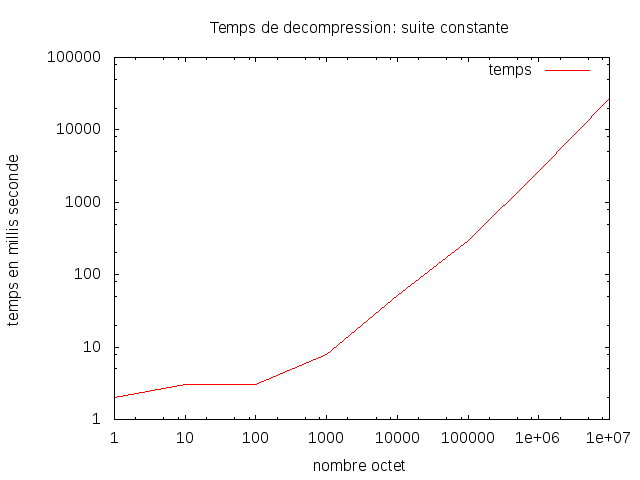
\includegraphics[width=7cm]{tempsDhC.png} & 
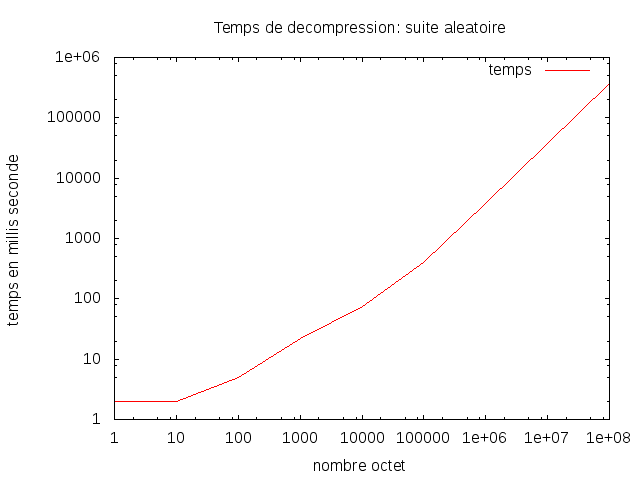
\includegraphics[width=7cm]{tempsDhA.png}
\end{tabular}
\subparagraph*{}
Le temps d'exécution pour la décompression de Huffman est linéaire. Ceci est notamment du à la lecture du fichier compressée, plus il est grand plus le nombre de caractère à traduire est important. 

Ce temps est très différent lorsqu’il s'agit d'une suite constante ou d'une suite aléatoire. Comme pour la compression il y a 2 explications à cela. La première est du à la lecture et au stockage en mémoire de l'arbre de compression, qui est nécessaire plus grand pour la suite aléatoire. La seconde raison est elle aussi liée à la lecture du fichier compressé. Comme il y a plus de caractère dans la suite aléatoire le code pour chaque lettre est donc plus grand, ainsi lors de la décompression il y a plus de caractère à lire dans le fichier compressé. Par conséquent, le temps de lecture de fichier est plus long.  

\paragraph*{}
\textbf{Temps d’exécution pour Lempel-Ziv}
\subparagraph*{}
\hspace{-2cm}\begin{tabular}{l | l}
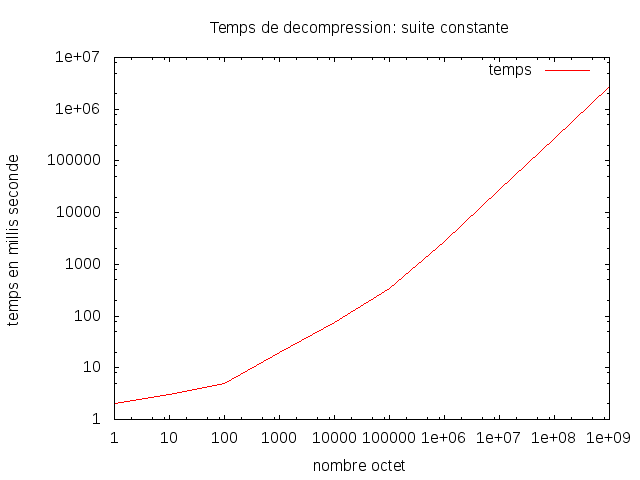
\includegraphics[width=7cm]{tempsDlzC.png} & 
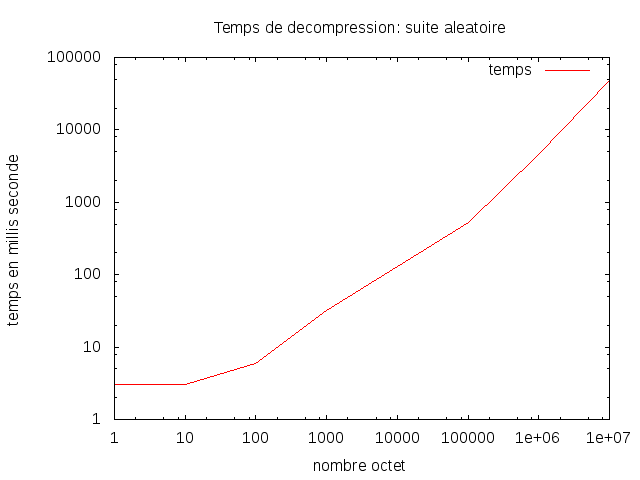
\includegraphics[width=7cm]{tempsDlzA.png}
\end{tabular}
\subparagraph*{}

Le temps d'exécution pour la décompression de Lempel-Ziv est lui aussi linéaire, pour les même raisons que celle évoquées précédemment.




\paragraph*{}
H vs LZ

\section*{Différences entre les algorithmes}
Dans cette dernière section, nous allons vous présenter un tableau avec plusieurs mode de compression et plusieurs type de fichiers. 
Nous expliquerons par la suite les différents taux de compression obtenues. 


\begin{flushleft}
{\renewcommand{\arraystretch}{2}
\begin{tabular}{|p{1.5cm}|p{1.5cm}|p{1.5cm}|p{1.5cm}|p{1.5cm}|p{1.5cm}|p{1.5cm}|p{1.5cm}|}
\hline
 & La bible (en anglais)  & Les Fleurs du Mal  & Au bonheurs des Dames & fichier PDF & musique  MP3 & image & vidéo\\
\hline
taille réélle (en octet)  & 883 158 & 180 199 & 952 753 & 198 931 & & & \\\hline
zip & 3,44 & 2,51 & 2,57 & 1,246 & & & \\
\hline
Gzip & 3,44 & 2,51 & 2,644 & 1,247 & & & \\
\hline
Bzip2 & 4,89 & 3,045 & 3,719 & 1,212 & & & \\
\hline
XZ & 4,649 & 2,826 & 3,323 & 1,261 & & & \\
\hline
Huffman & 1,725 & 1,688 & 1,747 & 0,998 & & & \\
\hline
Lempel-Ziv & 1,796 & 1,310 & 1,482 & 0,933 & & & \\
\hline

\end{tabular}
}
\end{flushleft}

\section*{Conclusion}



\end{document}